\documentclass{article}
\usepackage[utf8]{inputenc}
\usepackage{graphicx}
\usepackage{multicol}
\usepackage{caption}
\usepackage{vmargin}
\usepackage[numbers]{natbib} 
\usepackage[hidelinks]{hyperref}
\usepackage[charter]{mathdesign}
\usepackage{minted}
\usepackage{xcolor} % to access the named colour LightGray
\definecolor{LightGray}{gray}{0.9}

\def\ttdefault{blg}
\title{Signal Strength Detection Pattern Analysis for Classifying Suspicious Bluetooth Devices}
\author{Zhi Qu}
\date{July 18 2025}

\begin{document}

\maketitle
\section{Abstract}
BL(u)E CRAB is a program designed to address the growing threat of malicious tracking through Bluetooth Low Energy (BLE) devices, such as Apple’s AirTag. As BLE technology becomes more widespread, the risk of unauthorized surveillance increases. This project analyzes patterns in Received Signal Strength Indicator (RSSI) values to differentiate between suspicious and non-suspicious devices using sample data. The system parses, filters, and visualizes raw data into line graphs with RSSI values plotted over time. The analysis highlights devices that appear over extended periods of time and behavioral differences in suspicious devices. The program helps identify shared characteristics among flagged devices, providing insight into common traits. These findings lay the groundwork for a potential RSSI-based classification system to enhance BLE tracking threat detection.

    
    
\begin{multicols}{2}
    

\section{Introduction}
\subsection{BL(u)E CRAB}
BL(u)E CRAB is an app that detects signals from BLE devices to prevent stalking with these trackering devices. To do that, the app records RSSI (Received Signal Strength Indicator) values. Its aims are to address the threat that malicious tracking devices are being used to stalk people. \cite{conklin2025bl}

\subsection{Survey}
The developers of AirGuard, an app for Android and IOS users to detect Bluetooth trackers, conducted a survey. The survey aimed to assess the scale of the tracking issue and the effectiveness of protection measures. AirGuard users get a total of 400 warnings daily, although the number of devices that are false positives is unknown. \cite{turk2023stop}


\section{Others' Solutions}

\subsection{Apple}
In an effort to address the risk their cheap and accessible AirTags created, Apple phones' update included a warning system to alert the user to detected devices, along with an update on AirTags to sound an alarm when disconnected from their owner for time. This solution has various issues. For one, the software only detects devices that are disconnected from their owners. This leaves the possibility of physical tracking with the assistance of a device. For the safety of  normal AirTag users, the device MAC address rotates to avoid querying the server with one set address.
\cite{rescor2023def}


\subsection{AirGuard}

Airguard is a app developed to provide a tracker detection tool for Android users. The developers reverse engineered the safety feature that Apple developed for iOS. \cite{heinrich2022airguard} The program's flagging parameter includes being detecting over 30 minute duration per device. While 30 minutes seems reasonable, it is difficult to ensure that the time being tracked is accurate. When the malicious device is separated from the detector but remains with the victim's possessions, it may avoid flagging yet still stay near the victim. For example, the tracker is planted in a car but the drive times are short. In this case, when the user leaves their car, the detection time is stopped but the car's parking location would give away the user's location.



\end{multicols}
\section{Methodology}
\subsection{Datasource}
The data analyzed in this paper was collected by BLE-Doubt.\cite{briggs2022ble} The tests were conducted to replicate a tracking device maliciously planted on the user. The test has a set of suspicious devices.

\subsection{Reading Data Files}
First the MAC address, RSSI value, and time stamp are extracted from the dataset. the JSON file is a dictionary with detections key which contains keys for the "mac", "rssi", "t". In a straight forward manner, mac and rssi values could be collected in a loop for each detection log. The time required a more specified format to extract the information. 
\inputminted[firstline=31, 
lastline=34,
frame=lines,
framesep=2mm,
baselinestretch=1.2,
bgcolor=LightGray,
fontsize=\scriptsize,
]{python}{Final.py}


\begin{multicols}{2}
\subsection{Distinguish Devices}
After close examination of the output from the newly stored variables, it is clear that the detection data contains a distinct log for each device at every second detected. This creates a difficult situation where the information must keep the same index in their respective variables to produce the correct pairing. So first a separate list, fmac, is assigned each distinct value in mac, thus only storing one of each device. Then, in a loop for every device in fmac, every value in mac is checked for the same device address. based on the index of the matching device in mac, the rssi and time values are stored into a temporary list then stored as a list of lists.
\inputminted[
firstline=41, 
lastline=56,
frame=lines,
framesep=2mm,
baselinestretch=1.2,
bgcolor=LightGray,
fontsize=\scriptsize,
]
{python}{Final.py}

\subsection{Sort Based on Risk}
By cross referencing the logged device address with a dataset of known suspicious devices, all the corresponding RSSI and time values of that device are stored in a separate 2D array. When plotted, the suspicious devices are in red, and safe ones in blue. Seen in figures 3 and 4, the suspicious devices tend to have a higher RSSI value than safe devices. While that trend holds, the amount of overlap with non-suspicious devices varies. Some can be easily separated by a threshold, while others would produce many false positives if a horizontal threshold is implemented.
\begin{center}
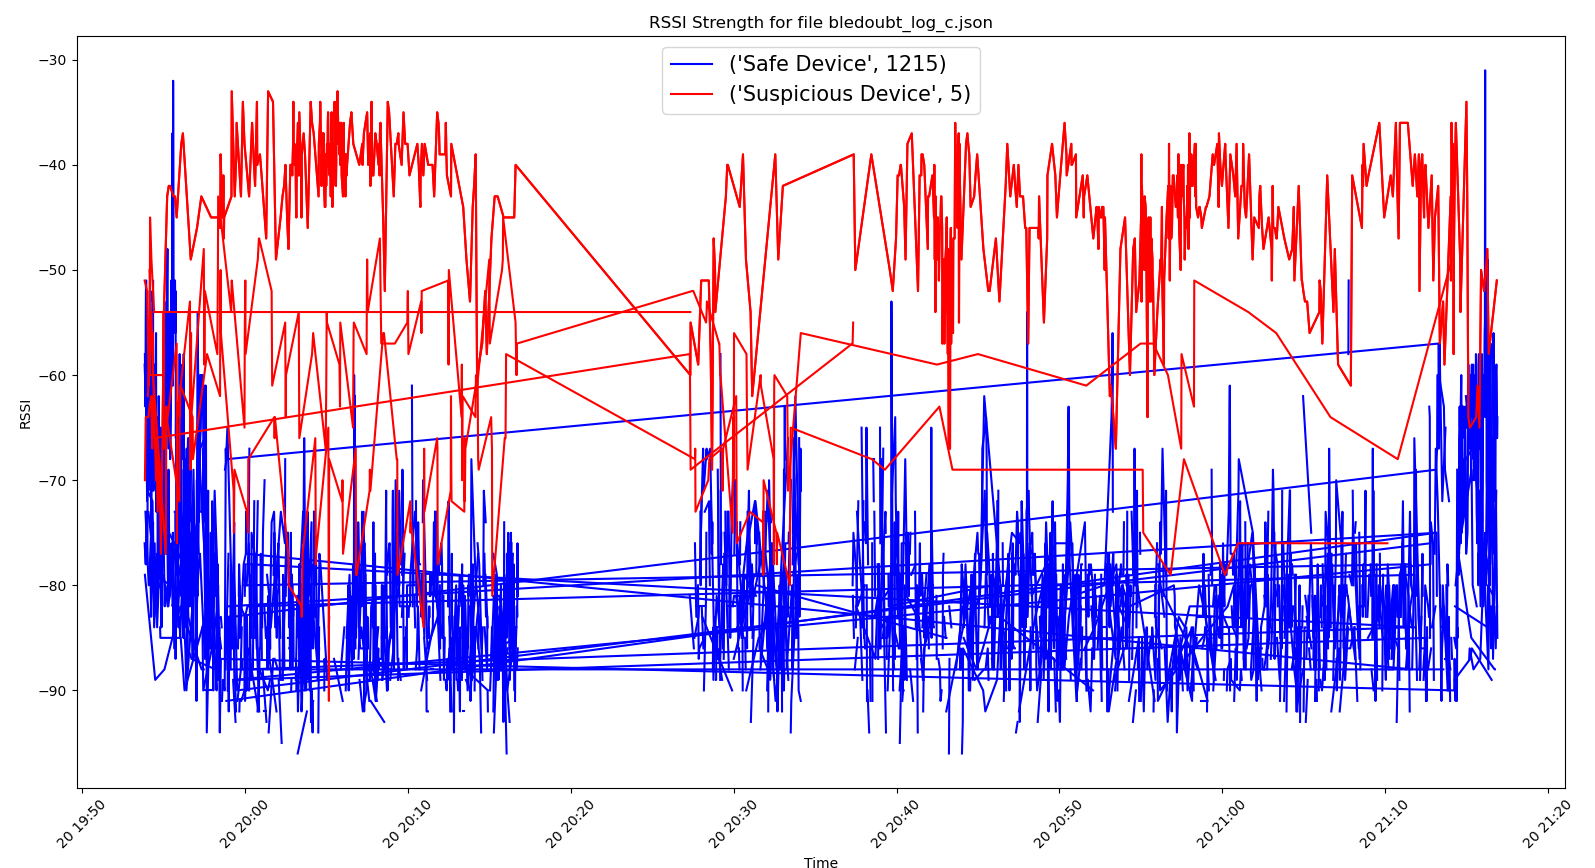
\includegraphics[width=1\linewidth]{Final-output-C.png}
Figure 1. Data file c
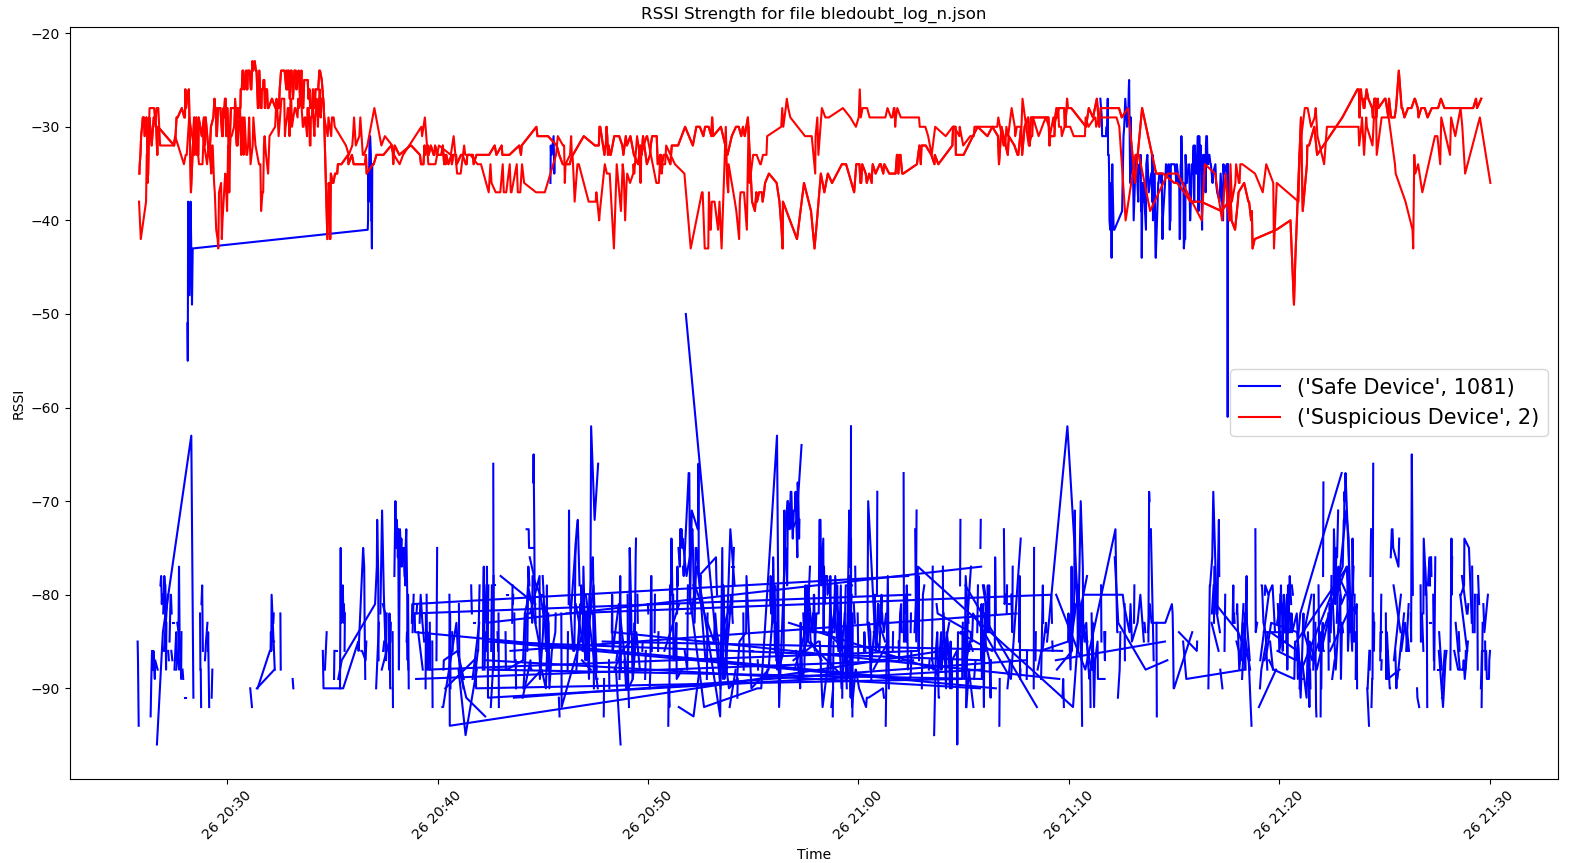
\includegraphics[width=1\linewidth]{Final-output-N.png}
Figure 2. Data file n
\end{center}
\end{multicols}


\subsection{Highlight Long Detections}
The exact difference between devices graphs can get lost with other device of similar signal strength as seen in figures 3 and 4. So to we added a higher parameter, the devices with significant periods of detection is separated, set to 60 seconds. The total amount of entries for one devices is the same the total seconds it was recorded for. When plotting, the normal data graph's the colors are changed to lighter shade of red and blue while the devices with a significant detection time frame remains pigmented. \footnote{all suspicious devices in all logs were flagged with significant duration.}
\inputminted[firstline=122, 
lastline=131,
frame=lines,
framesep=2mm,
baselinestretch=1.2,
bgcolor=LightGray,
fontsize=\scriptsize,
]{python}{line-label-time.py}

\begin{center}
    Figure 3. the highlighted version of data file c. 
    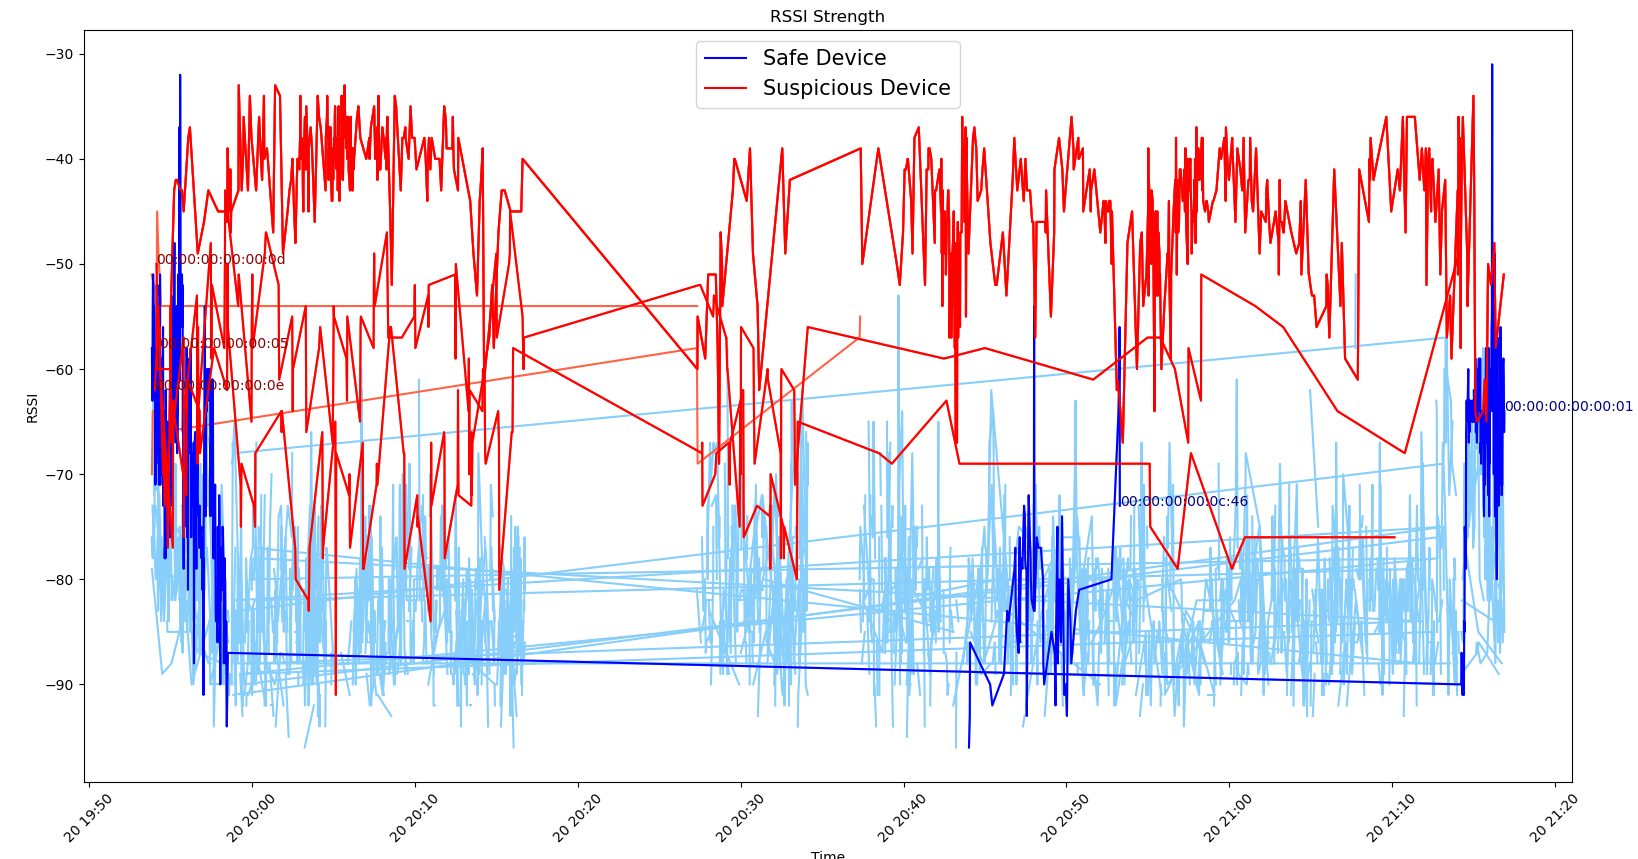
\includegraphics[width=1\linewidth]{line-lable-time.png}
\end{center}


\subsection{Compare Time of Day}
To streamline that repetition of data set plotting, a new function "plot" is created to take in unique datasets in the main function.
    

\inputminted[
firstline=89,
lastline=99,
frame=lines,
framesep=2mm,
baselinestretch=1.2,
bgcolor=LightGray,
fontsize=\scriptsize,
linenos
]{python}{time-of-day.py}




\begin{multicols}{2}

\section{Discussion}
All suspicious devices are flagged as significant in the detection time. It is possible that these pattern is a trend from the test set up. In real world circumstances, other than person devices, a planted tracker will be detected for a significant amount of time. At the same time, the duration of the test was between 15 minutes to 1 hour 30 minutes, which can skew the overall time significance of the suspicious devices.
\begin{center}
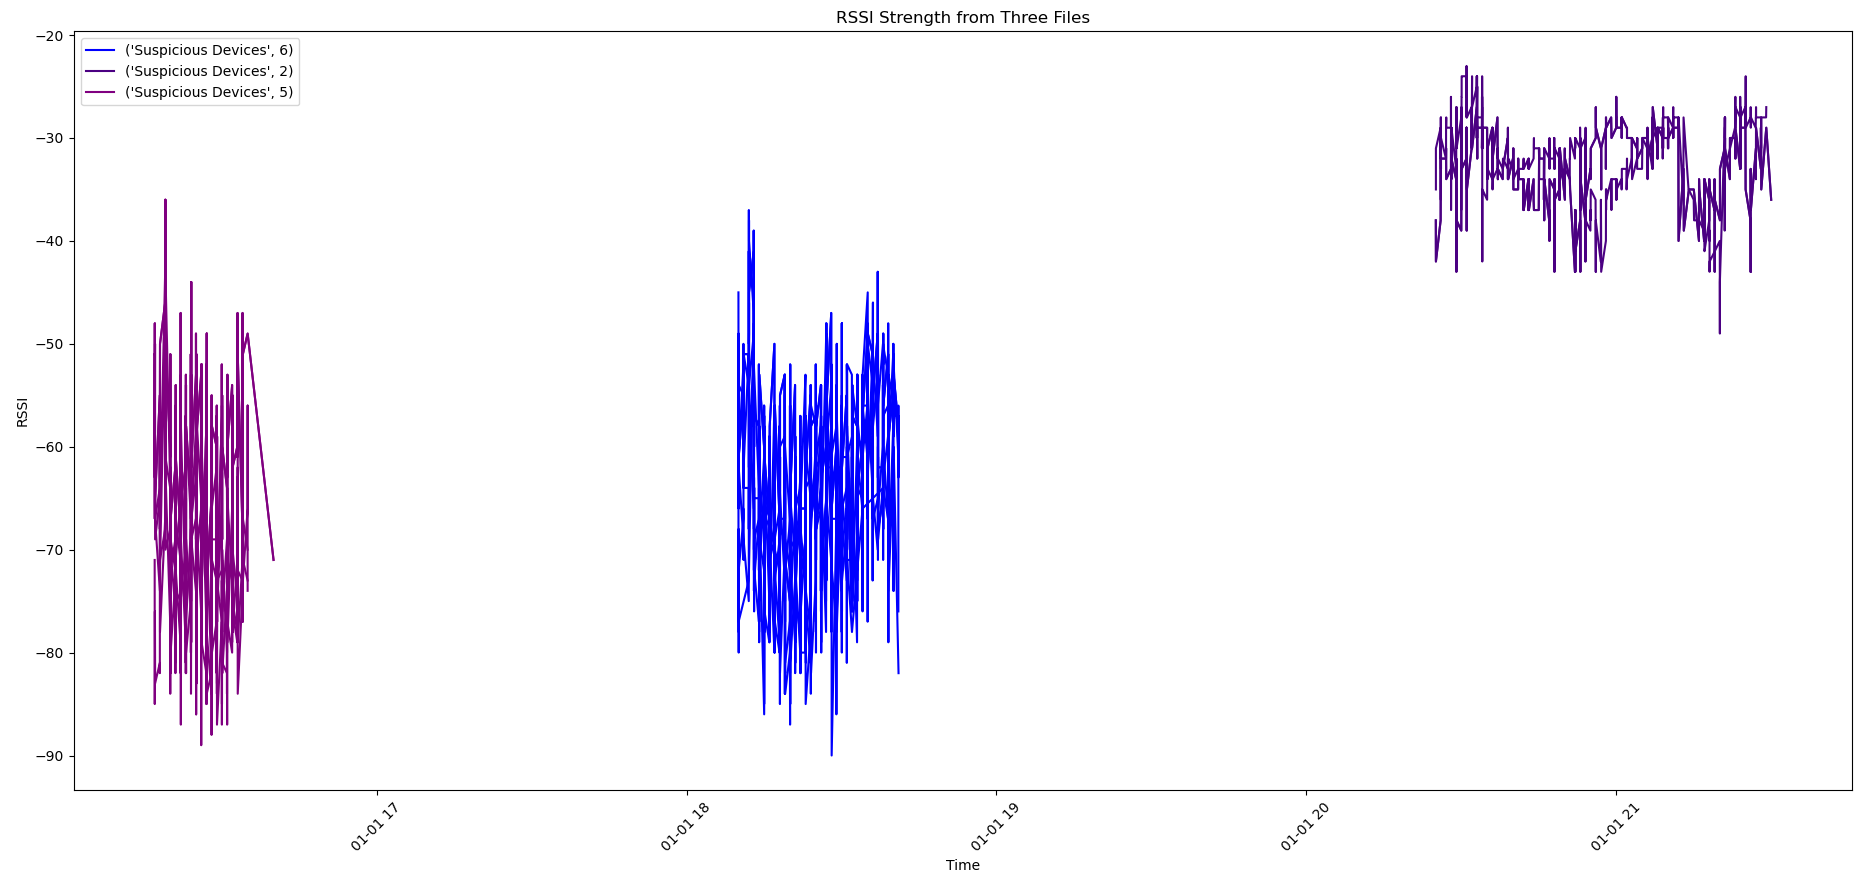
\includegraphics[width=1\linewidth]{three-g-n-j.png}
Figure 4. file g and n with file j in blue
\end{center}
No distinct trend could be identified from the assessment of different times of the day. While some of the data sets graphed together present a possible pattern, it is more likely that the difference in RSSI strength comes from where the tracker was placed in relation to the detector.
\begin{center}
    
Figure 5. Files g and n with file a in blue
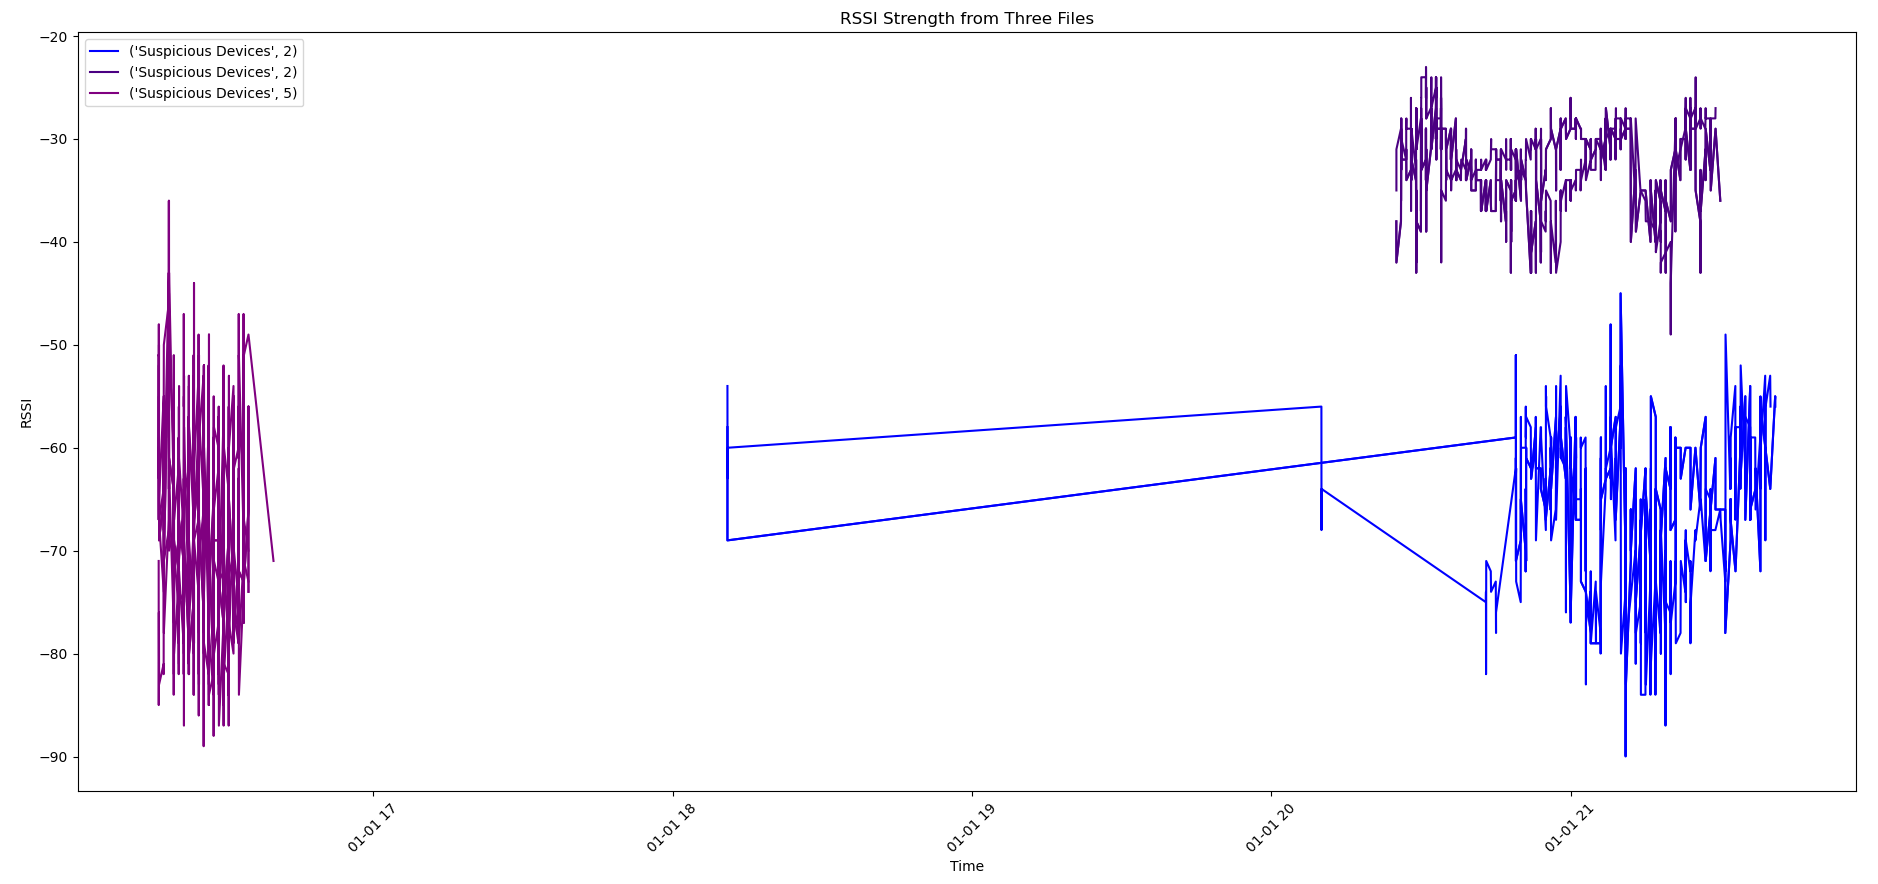
\includegraphics[width=1\linewidth]{timeofday_a_g_n.png}

\end{center}


\section{Conclusion}
The program is able to produce easily readable graph and provide a general understanding of the device distribution based on RSSI values and time. Suspicious devices tend to show higher RSSI values and all detected for a significant amount of time(60 seconds). As a user travels they will encounter many safe devices that belong to normal crowds which will not get very close as a reflection of human behavior but suspicious devices are placed on the user thus is closer and has stronger signals. Suspicious devices have long detection time: may be due to the design of the testing The difference of RSSI values seen on time of day graphs is more likely to be related to the planted location of the suspicious trackers


\subsection{Limitations}

\begin{itemize}
    \item The data input must be in the same format as the sample data, or the information extraction will result in an error.
    \item Individual data points are often difficult to see, meaning that the observations are high-level generalizations rather than confirmation of a precise pattern. Thus, applying a definite threshold may not be effective.
\end{itemize}
\end{multicols}
\newpage



\bibliographystyle{IEEEtranN}
\bibliography{refs}


\end{document}